%%%%%%%%%%%%%%%%%%%%%%%%%%%%%%%%%%%%%%%%%
% Introduction
%
% $Date$
% $Revision$
% $Author$


\chapter{Introduction}\label{chap:introduction}

Modern software applications are often complex and have to fulfill a large set of functional and non-functional requirements. The internal behavior of such large systems cannot easily be determined on the basis of the source code. Furthermore, existing applications often lack sufficient documentation which makes it cumbersome to extend and change them for future needs. A solution to these problems can be dynamic analysis based on application-level monitoring, which allows to log the behavior of the application and to discover, for example, application-internal control flows, calling dependencies, and method response times.

Dynamic analysis can help in detecting performance problems and faulty behavior, capacity planning, and many other areas. The \Kieker{} framework provides the necessary monitoring capabilities and comes with tools and libraries for the analysis of monitored data. \Kieker{} has been designed for %
continuous monitoring in production systems inducing only a very low overhead. Further information on the overhead caused by \Kieker{} is provided at \url{http://kieker-monitoring.net/overhead-evaluation/}.
%, and offline evaluation of monitored data for a deeper inspection of the application's behavior and runtime architecture.

Please note that this document is aging.
We have started to transfer its content to our wiki \url{https://kieker-monitoring.atlassian.net/wiki/discover/all-updates}.

%%
\section{What is \Kieker?}\label{sec:kieker}



\Kieker{} is a Java-based application performance monitoring and dynamic software analysis framework~\cite{KiekerICPE2012}. %
Monitoring adapters for other platforms, such as Visual Basic~6~(VB6), .NET, and COBOL, exist as well.%
\footnote{\href{http://kieker-monitoring.net/support/}{Contact us} directly if you are interested in \Kieker{} support for other platforms} %
Figure \ref{fig:KiekerComponentDiagram} shows the framework's composition based %
on the two main components \KiekerMonitoringPart{} and \KiekerAnalysisPart{}. %

% This is the component diagram of Kieker (the satellite).
\begin{figure}[H]\centering
\includegraphics[width=0.96\textwidth]{images/kiekerComponentDiagram-woCloud-bw-w-record-newNames-withTraceAnalysis-colors}
\caption{Overview of the framework components}
\label{fig:KiekerComponentDiagram}
\end{figure}

\noindent The \KiekerMonitoringPart{} component is responsible for program instrumentation, data collection, and logging. Its core is the \class{MonitoringController}. %  which %
%receives the monitoring data in so-called monitoring records from monitoring probes, and writes these %
% receives the monitoring data and passes it to the configured monitoring log writer. %
%
The component \KiekerAnalysisPart{} is responsible for reading, analyzing, and visualizing the monitoring data. Its core is the \class{AnalysisController} which manages the life-cycle of the pipe-and-filter architecture of analysis plugins, including monitoring readers and  analysis filters.

The monitoring and analysis parts of the \Kieker{} framework are composed of subcomponents which represent the different functionalities of the monitoring and analysis tasks. The important interaction pattern among the components is illustrated in Figure~\ref{fig:KiekerCommunicationDiagram} but will be explained furthermore throughout the course of this user guide.

\vspace{1cm}

% This image shows the communication diagram of the different components.
\begin{figure}[H]\centering
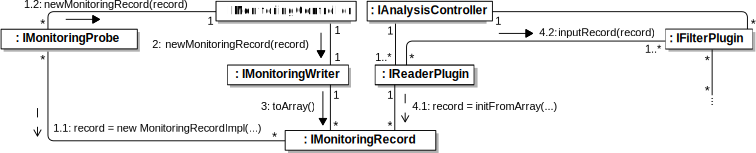
\includegraphics[width=1\textwidth]{images/kiekerCommunications-revisedReArranged-woMonitoringLog-bw-newNames}
\caption{Communication among \Kieker{} framework components}
\label{fig:KiekerCommunicationDiagram}
\end{figure}

% \vspace{1cm}

% Notify-tag because it is explained how Kieker works.
% avh: removed
\noindent The monitoring probes create the monitoring records containing the %
monitoring data and deliver them to the monitoring controller. %
The monitoring controller employs the monitoring writers to write these %
monitoring records to a monitoring log or stream. %
For analyzing purposes, monitoring reader plugins read the records from the %
monitoring log/stream. These records can then be further processed by a %
configuration of additional filter and repository plugins, inter-connected via input and output ports. %


\section{Kieker is Recommended by the SPEC Research Group}

In 2011, Kieker was reviewed and accepted for distribution as part of the SPEC Research %
Group's repository of peer-reviewed tools for quantitative system evaluation and analysis. %
See \url{http://research.spec.org/projects/tools.html} for details.

